\chapter{Concept and Design}
\label{cha:conceptanddesign}

As stated in the research statement, the goal of this thesis is to come up with a solution that solves the unpaid content problem. During the first phase of this research, several opportunities are explored. This chapter gives a chronological overview of these explorations and describes the final model in detail.

In the beginning, the main focus laid on privacy issues that are coming with the use of ad networks. In order to solve this issue, a concept is created in which the tracking and profile building moved from the ad network to the browser of the user. By using such an approach, the ad network does not know your browsing history and might even benefit from the new approach, because the browser is able to build a profile that is much more accurate. 

The problem with this concept has been actively researched. For example, it is implemented in the Privad system, which can be found in section \ref{sec:privad} and the Brave browser, which is discussed in section \ref{sec:brave}.

\label{sec:uaps}
The second concept goes one step further. This concept is not about replacing the ad network with a privacy friendly alternative, but making the entire ad network obsolete. As discussed in Chapter \ref{cha:relatedwork}, the problem with ad networks is that it is one of the few revenue models that actually works on the internet.

Several commercial experiments are performed using micropayments, however, as stated in Chapter \ref{cha:relatedwork}, very few of them are successful. Mainly because of the mental transaction costs that comes with the purchase of online content. In order to solve this issue, the concept of automated payments is introduced. This approach applies the advantage of web advertisements (no browsing interruption) with the benefit of micropayments (no ads). It might also be explained as a fair ad blocker. No ads, while taking care of the revenue of the publisher. The goal of this concept is to offer such a system with as minimal configuration as possible.

\newpage

\begin{figure}[h!]
  \center
  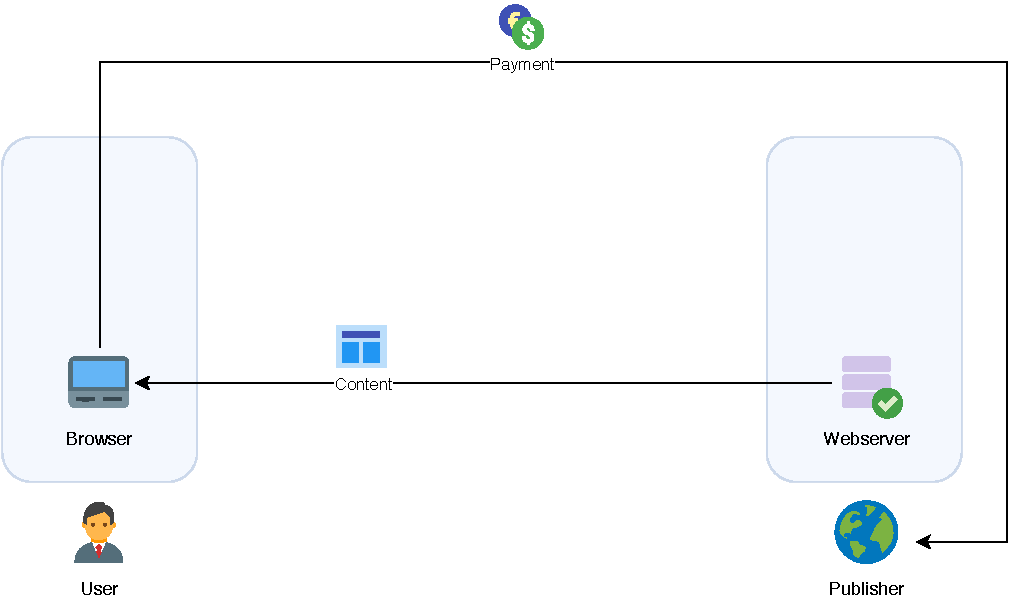
\includegraphics[width=12cm]{images/concept.pdf}
  \caption{Proposed concept overview}
\end{figure}
\vspace{2em}

Concept: \textit{Distribute a small amount of money over the publishers behind the websites you visit and hide the advertisements}

\vspace{2em}

Potential challenges:
\begin{enumerate}
  \item How to keep the configuration as minimal as possible?
  \item What design can be applied to operate the system in a decentral way?
  \item How to determine the amount of contribution?
  \item How to prevent fraud?
\end{enumerate}


In order to stick to the zeroconf (zero or minimal configuration) principle, the system should work out of the box, without any configuration. To do so, this concept uses WebRTC. WebRTC is a system that enables two browsers to create a peer to peer connection to each other.

This concept assumes that there is a system running that handles all the automated payments to the publisher. The first problem that needs to be solved is: how does the website communicate with the system. Installing an add-on in the browser would violate the zeroconf principle, so this approach uses WebRTC as a message bus. The reason why WebRTC is chosen, is that WebRTC makes it possible for browsers to communicate with each other. Besides, it is also possible for different websites to communicate in the same browser. Normally, this is not so easy because every website runs in a sandboxed environment. For example, if \textit{derspiegel.de} wants to communicate with a system on \textit{payjs.io}, that is only possible if there is a link between both websites, such as an iframe or if one of the websites opened a tab to the other one. 

WebRTC connects to an IP address, so what happens if it is connected to localhost? Is it possible to let two websites communicate without a link between them? The WebRTC is indeed able to connect to localhost, but in order to do so, a handshake is needed \cite{dutton2013webrtc}. This handshake, however, is not specified in the WebRTC protocol. This means the system can implement its own way of doing so. WebRTC-systems that are applied on the internet are mostly relying on a signaling server, which forwards the handshake. 

During this research, several experiments are performed using WebRTC. Unfortunately, it turned out that it is not possible to connect two websites within one browser directly. A signaling server that is run by a third party stays neccesary. This would introduce a privacy problem, because the third party would be able to find out which publisher is visited from which IP address. Therefore, considering this thesis, the concept is abandoned at an early stage.

The approach above, however, does not include any form of payment. In the first stage, the scope is limited to a universal payment system, without taking care of the payment itself. It is assumed that there is a cryptocurrency solution that can be attached to the universal payment system.

Fortunately, parallel to this research, a micropayment solution based on the Bitcoin blockchain is being actively developed. This so-called Lightning Network is discussed in section \ref{sec:lightning} in more detail. The goal of this system is to provide instant micropayments at minimal costs, which is ideal for an automated payment solution.

From the concept point of view, the payment part is a matter of communicating with an API. Nonetheless, due to some issues with the Lightning Network, it is not yet ready. One of the main disadvantages of the Lightning Network is that it is not possible to send a transaction to an address directly. By design, a payment should be requested by issuing an invoice. This invoice is written according to a standard format and can be paid using any Lightning Network client. This invoice-based structue is suboptimal for the usecase that is needed for this research.

As it was shown, the concept where WebRTC is applied in order to let the publisher communicate with the system, is not viable. Therefore, this research is extended to other approaches. One approach that is used by other websites to communicate with the users' computer is by running a webserver. This webserver can be accessed from any website by connecting to localhost. For example, the popular video conferencing application Zoom uses this approach so that the application gets opened when a user visits a meeting URL \cite{zoomwebserver}.

As this concept is built in combination with the Lighting Network, there needs to be an application running on the users' computer anyway. This makes it possible to develop one service that needs to be installed, which acts like both a lightning network client and an interface on localhost to the website that requests a payment.


\section{Wallet address listing}

As described in the Lightning Network concept, there is a possibility to send micropayments to a publisher. The challenge in this case is, how to communicate the wallet address of the publisher to the users' computer? Of course, it is possible to just store it somewhere in a javascript variable. A potential security flaw in this approach is that some websites are executing user generated content, for example: it is possible to host a website with javascript content on \textit{github.io}. In that case it is not desirable that a fraudulent party spams javascript snippets over the internet that asks for an automated payment without contributing to valueable content. 

One aspect of websites is barely modified by user generated content: DNS records. DNS records are only modifyable by the owner of the domain name, which, in most cases, is the publisher. One way of storing information in DNS records is to just create a subdomain that contains the content: in this case, the wallet address of the publisher. 

Fortunately, the DNS specification also features a so-called TXT record. This is a record that does not affect the way the domain name is resolved. However, it can be queried and used by other applications. For the automated payment design, the TXT record is used by the system to provide the wallet address of the publisher, so that it cannot be modified by someone else, other than the owner of the domain name. 

\section{Self-signed, DV, OV and EV certificates}

One of the problems with an automated payment system is: how can be determined if a publisher is trustworthy? For example: what happens if some malicious publisher buys a bunch of domain names and opens 50 tabs on the users' computer? Does the system make a payment to all 50 domains? 

One approach would be to assign one party that is able to determine which publisher is trustworthy and which one is not. This would violate the decentral principle of the concept and is therefore not desirable. Another approach that is discussed is to calculate some kind of score, such as pagerank, and use this score to value the credibility of the publisher. Based on this credibility, a payment might be made or might be adjusted. For example: the domain name \textit{spiegel.de} has a pagerank score of 8/10 where \textit{gartenforum.de} has a pagerank score of 3/10. This ranking, however, does not indicate the trustworthyness of a publisher. There is no legitimate reason to pay more to a big publisher than to a small independant content creator. 

Fortunately, there is already a worldwide decentral system in place that validates credibility of websites: SSL certificates. SSL certificates, that are needed in order to establish an encrypted connection to a website, are also applied to make sure that the user is communicating with the website that it pretends to be. In order to understand this concept, a short introduction to the different types of certificates and architecture is given. 

First, a certificate needs to be issued by an authority. The credibility of the certificate is based on the credibility of the issuer. If some publisher issues the certificate by themselves, it is called a self-signed certificate and this provides no credibility other than that the connection is encrypted. There is, however, no guarantee that the party on the other end of the line is the party they are pretending to be. If the issuer is a trusted party, the certificate is called a certification authority (CA). These CA's are trusted by the browser or SSL library, and they are doing a couple of background checks before they are issuing a certificte. The level of background checks depends on the type of certificate. 

The least secure type of CA certificate is the Domain Validation (DV). These certificates are available for free and can be used by anyone that owns a domain name. Therefore, a DV certificate does not say anything about the credibility of the publisher. A fraudulent party is able to register a bunch of domain names and also apply for certificates.

A more secured certificate is the Organization Validation (OV), also known as a High Assurance certificate. With this type of certificate, the issuer does some background checks in advance. These background checks include the verification of the information in a third party database, such as a companies house. One other aspect of these certificates is that they are not free, which means that it is less easy to register a bunch of domain names. Major publishers, such as \textit{spiegel.de} are using these OV certificates.

As an extension to the OV certificate, there is an Extended Validation certification. In the past, this type of certificate was popular amongs banks and government agencies, because it showed the name of the legal entity in the browser when such a certificate was used. EV certificates are even more expensive, as the background checks are comprehensive.

These aspects of SSL certificates are very valueable in order to determine the credibilty of a publisher. The default setting of the universal payment solution will be that automated payments are only made to publishers with an OV or EV certificate.



\section{Revenue distribution}

One of the challenges of this concept is to pay a fair share to the publisher. How to determine the amount that is contributed? The general idea is that the amount should be in the same order of magnitude as the revenue when an online advertisement is displayed. In online advertisement jargon such a display is called an impression. The price of such an impression is determined as Price-per-mille (CPM), the price for 1,000 impressions. If a user clicks on an advertisement, the fee is called the cost-per-click (CPC). The amount of users that clicks on the advertisment is expressed in click-through-rate (CTR) \cite{evans2009online}. For the Google Display Network (which also includes services like Gmail), the following average numbers are available for the first quarter of 2018\cite{cpmgoogle}: 

\begin{itemize}
  \item CPM: 2.80 USD
  \item CPC: 0.75 USD
  \item CTR: 0.35\%
\end{itemize}

\noindent With this data, it is possible to calculate the average revenue per served ad, which is:

\begin{equation}
\cfrac{CPM}{1000} + CTR \times CPC = \cfrac{2.80}{1000} + 0.75 \times 0.0035 = 0.005425 ~\text{USD}
\end{equation}

\noindent In order to estimate the online ad revenue per user per month, this revenue is multiplied with the average amount of ads that are served to a user, which is around 1,700 \cite{papadopoulos2018cost}. 

\begin{equation}
  \text{revenue per ad} \times \text{impressions per month} = 0.005425 \times 1,700 = 9.22 ~\text{USD}
\end{equation}
This results in an average revenue per internet user of 9.22 USD per month. This, however, does not include the margin of the advertising networks, which is somewhere between 20 and 50 percent. For the Google Display Network it is 32 percent \cite{googlefee}. If we subtract this fee from the calculation above, the remaining profit for all publishers is:


\begin{equation}
  \text{revenue per month} \times (\text{1 -- ad network fee}) = 9.22 \times (1 - 0.32) = 6.26 ~\text{USD}
\end{equation}


This net profit per internet user per month forms the basis for the pricing model of this concept. By using these numbers, there should be no difference between targeted advertising and this concept in terms of revenue for the publisher.

The next question that needs to be answered is: how to distribute this amount over the publishers in a fair manner?  

The simplest way would be to do $\cfrac{c}{n}$, where $c$ is the contribution per month and $n$ is the amount of publishers. The problem with this approach is that this cannot happen on the fly. $n$ is unknown during the visit of the website. One approach would be to just pay all the publishers once at the end of every month, but that would introduce a lot of risk and prevent the system from making contributions in real time. 

Another approach would be to just make an assumption on $n$, and pay out to the publishers accordingly. If $n$ is reached, the payments will stop. This system is still not ideal, because such assumption is hard to make.

The solution that is presented in this concept, uses a hybrid form of both approaches described above. The system will set a budget per day, based on the calculations above. Lets call this budget $b$. If the user visits a website, the contribution to that particular website will be $\frac{1}{10}$ of the budget. For example: lets say the budget is 20 cents per day. The users visits an article on The Guardian, $\frac{1}{10}$ of the budget, which is 5 cents, is sent to the guardian. Afterwards, the users visits a Wikipedia article, $\frac{1}{10}$ of the budget is sent to Wikipedia. However, only 18 cents of the budget is left. Now $\frac{1}{10}$ of 18 cents, which is 1.8 cents, is sent to Wikipedia. As time passes, the budget is topped up every minute by $\cfrac{b}{1440}$.

Using this approach, the user will never overspend the budget $b$, but is still able to contribute to every website that he visits. One concern could be that websites that are visited in the beginning in the browsing session are rewarded better than websites that are visited at the end of the browsing session. Nonetheless, the browsing behavior of every user is different. In the end, these differences might equal out.

One other concern about this approach is the payment is based on pageviews. If a user is browsing 20 different Wikipedia articles, that would result in the same revenue as the same user using a search engine 20 times. Of course, it is possible to limit the contribution to only one contribution per publisher per day. But as this concept tries to be an alternative to online advertising. Online advertising generates revenue based on impressions, which means that spending more time on a website generates more revenue. Therefore, this aspect of the revenue is also implemented in this concept. 

Unfortunately, research on this approach did not result in any terminology or a basic mathematical principle. From now on, this approach will be called fractional contribution. 
